\section{EVALUATION}
\label{sec:eval}

\begin{figure}[!t]
  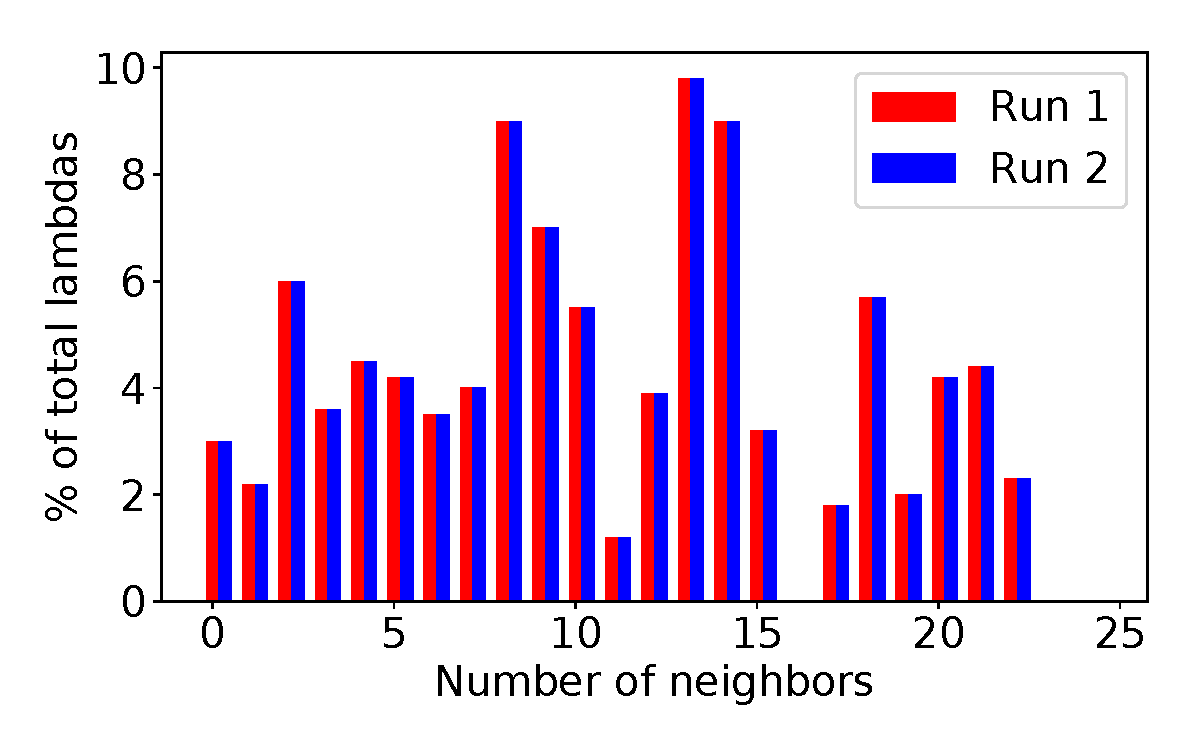
\includegraphics[width=.99\linewidth]{fig/correlation.pdf}
  \caption{Shows the fraction of lambdas by the number of neighbors they saw for two 
  independent runs that use same set of underlying AWS containers. The perfect correlation 
  shows that both runs depict the colocation status of those containers regardless of the 
  lambdas that ran on them, providing an evidence for the correctness of our technique.
\label{fig:correlation}}
\end{figure}

In this section, we evaluate the effectiveness of our co-residence detection
technique with respect to reliability and scalability, the desirable detection
properties mentioned in section~\ref{sec:methodology}.  We run all of our
experiments with AWS lambdas~\cite{awscloud}. Though we decide to focus on one
of the cloud providers, we have previously shown in section \ref{sec:methodology} 
that this covert channel exists on the other clouds, and thus these experiements can be
replicated on their serverless functions as well. We use C++ runtime in AWS 
lambdas as it allows pointer arthmetic that is required to access the covert channel.

\subsection{Setup}
\label{subsec:expsetup}
For each experiment, we deploy a series of instances from an AWS lambda
account. Once deployed, each instance participates in the first phase of the
protocol as noted in section \ref{sec:protocol:complexity}, thereby learning the
largest ID of their neighbors. As bit-flip errors are possible, we repeat the
same phase for two more (independent) "rounds" and take the majority result to
record the ID seen by this instance.  If all three rounds result in different
IDs, we classify this instance as erroneous and report it in the error rate. We
group all the instances that saw the same ID as successful and neighbors. We
repeat the experiments for different lambda sizes and in various cloud regions.


\subsection{Reliability}
We consider the results of the technique reliable when 1) most of the deployed
instances successfully see the same result in majority of the independent rounds
(indicating lesser bit-flip errors) and 2) the resulting co-located groups we
see match the ground truth.  For 1, we ran an experiment with 1000 AWS lambdas
and compared the error rate across different lambda sizes (the error rate
indicates the fraction of these 1000 lambdas that did not have a majority
result). From Figure \ref{fig:errorrates}, we can see that smaller lambdas see
lot more errors. This is expected because, as discussed in section
\ref{sec:method:noise}, these lambdas experience lossy communication making it
harder for our technique to sense contention. The lambdas above 1.5 GB, though,
see a 100\% success rate.   

\textbf{Correctness} 
To determine correctness, we require ground truth on which instances are
co-located with one another, which we are able to ascertain by utilizing an AWS
caching mechanism. After execution, AWS caches the lambda containers to reuse 
them\cite{awscontainerreuse} for repeat lambdas and mitigate
"cold start" latencies. For C++ lambdas, we found that the data structures
declared in the global namespace are tied to containers and are not cleared on
each lambda invocation, so we can use a global array to record all the lambdas
that were ever run in a particular container. This means, for a given lambda, we
can precisely tell all the lambdas that previously ran in the same container
(aka predecessors).  Using this, we are able to validate that identical
experiments repeated within minutes of one another will use the same set of
underlying containers for running the deployed lambdas. Since lambda co-location
is essentially co-location of their containers, and given that containers
persist across experiments that are executed within minutes of one another,
lambda co-location results must agree with the co-location of their underlying
containers for true correctness.


\begin{figure}[!t]
  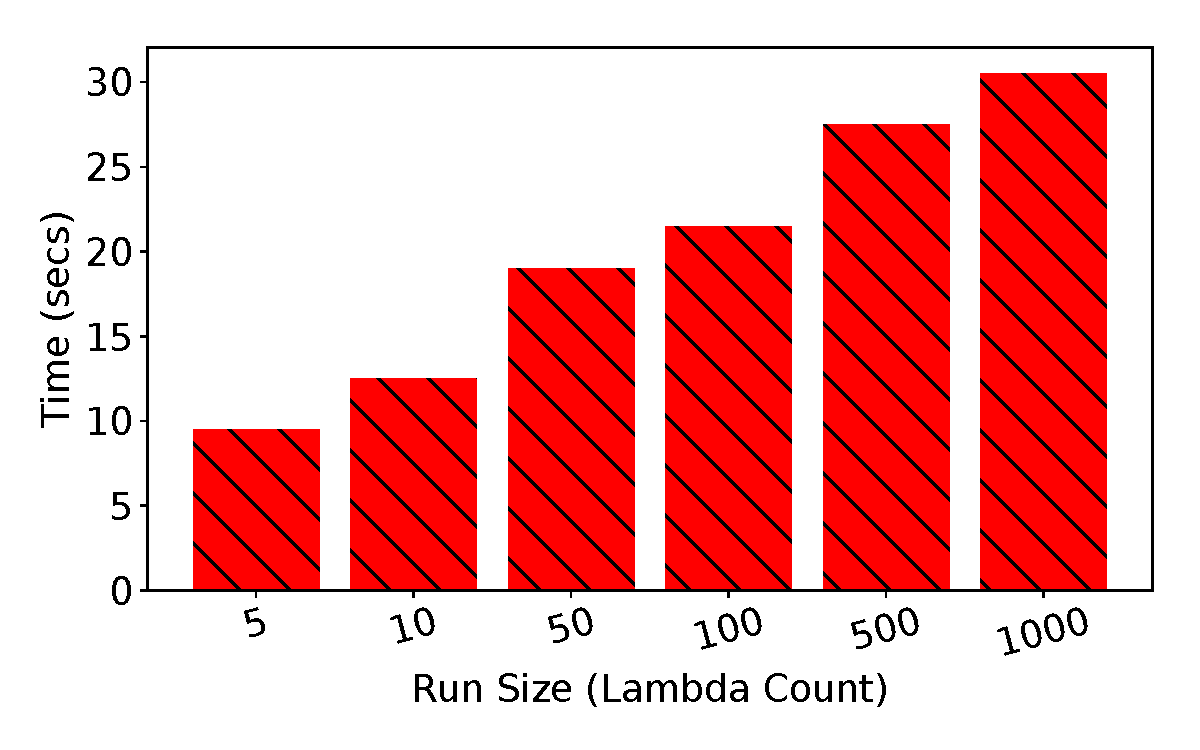
\includegraphics[width=.99\linewidth]{fig/runtimes.pdf}
  \caption{Shows the average runtime of a lambda for co-location runs of different sizes. 
  The run time increases logarithmically with the number of lambdas as it is proportional to
  the number of bits required to uniquely identify all the lambdas. \todo{Get real data.}
\label{fig:runtimes}}
\end{figure}

To demonstrate this principle, we run an experiment with 1000 1.5GB cold-started
lambdas (ID'ed 1 to 1000) in one of densest AWS regions (AWS MiddleEast), which
resulted in many co-located groups.  We repeat the experiment within a few
seconds, thereby ensuring that all 1000 lambdas are warm-started on the second
trial (i.e., they use the same set of containers from the previous experiment).
For each co-located group of lambdas in the latter experiment, we checked
whether their predecessor lambdas (that used the same set of containers) in the former one 
formed a co-located group a well. \amirian{a bit lost here} \anil{how about now?} 
We observed that while the lambdas that used a set of containers differ across 
both experiments, the results of these experiments agree perfectly on the continer 
colocation. Figure~\ref{fig:correlation} shows that both experiments saw
the same number of groups of different sizes. This proves the correctness of
our co-location results.

\subsection{Scalability}
One of the key properties of this technique is its execution speed.  Since
communicating each binary bit of the ID takes one second, we are able to scale
the technique logarithmically with the number of lambdas involved.
Figure~\ref{fig:runtimes} shows this principle for experiments involving
different number of lambdas. For example, in an experiment with 10000 lambdas,
each lambda can find its neighbors within a minute of its invocation, leaving
ample time to use this information for nefarious purposes. The logarithmic scale
of our method also indicates that the cost per lambda scales logarithmically,
making neighbor detection cost-effective.



% Figures from the next section
% Moved here for formatting

\begin{figure}[!t]
  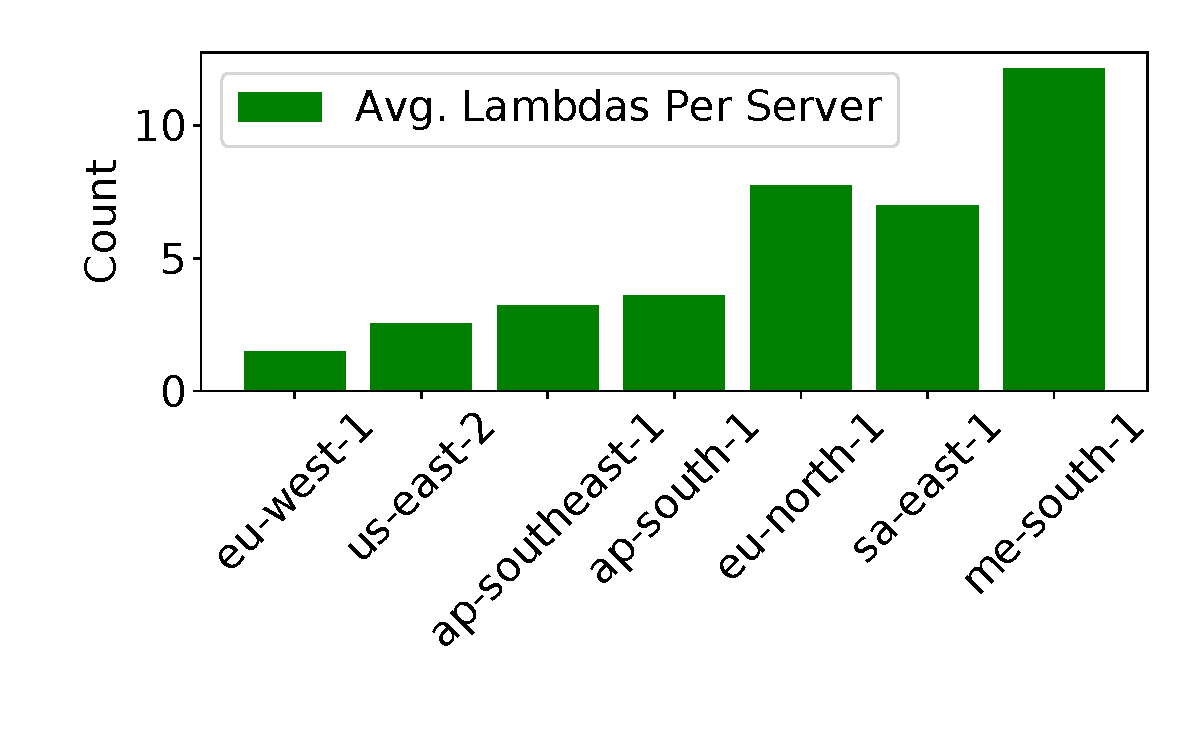
\includegraphics[width=.99\linewidth]{fig/density.pdf}
  \caption{Shows the average number of lambdas per server i.e., colocation 
  density seen in various AWS regions for a 1000-lambda run.
\label{fig:density}}
\end{figure}

\begin{figure*}[!t]
\begin{subfigure}{.33\textwidth}
  \centering
  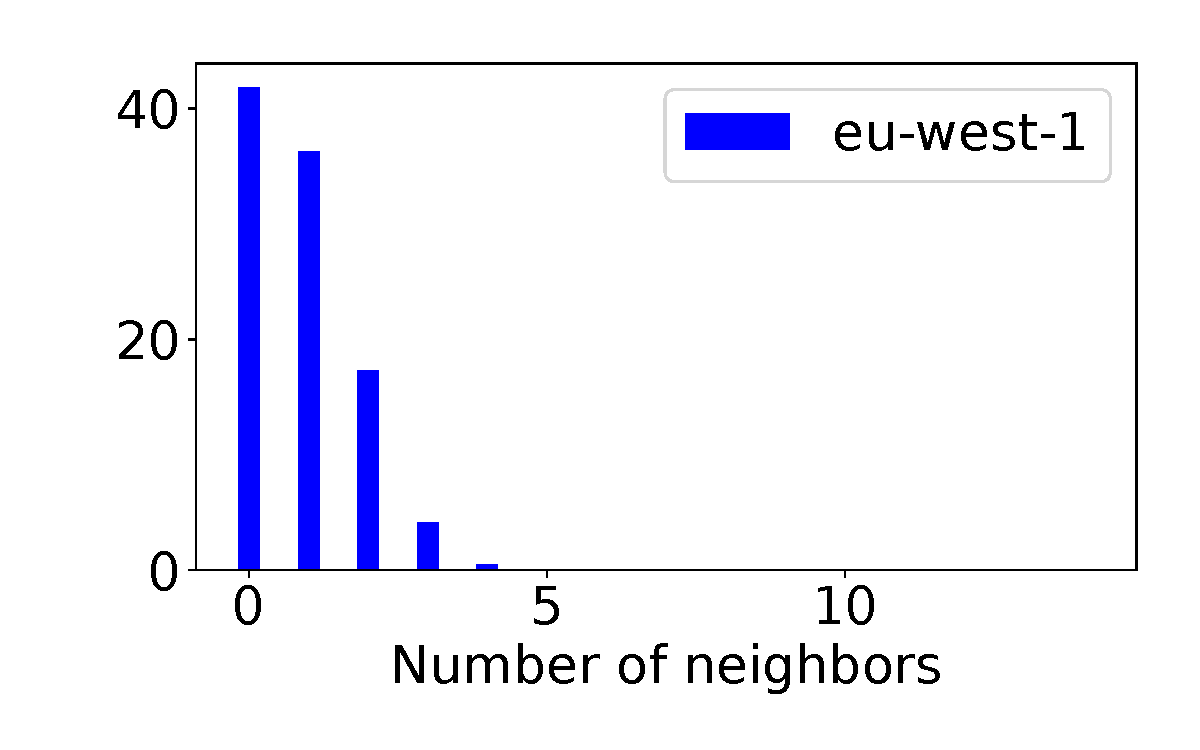
\includegraphics[width=.99\linewidth]{fig/colocation-eu-west-1.pdf}
%   \caption{1a}
%   \label{fig:sfig1}
\end{subfigure}%
\begin{subfigure}{.33\textwidth}
  \centering
  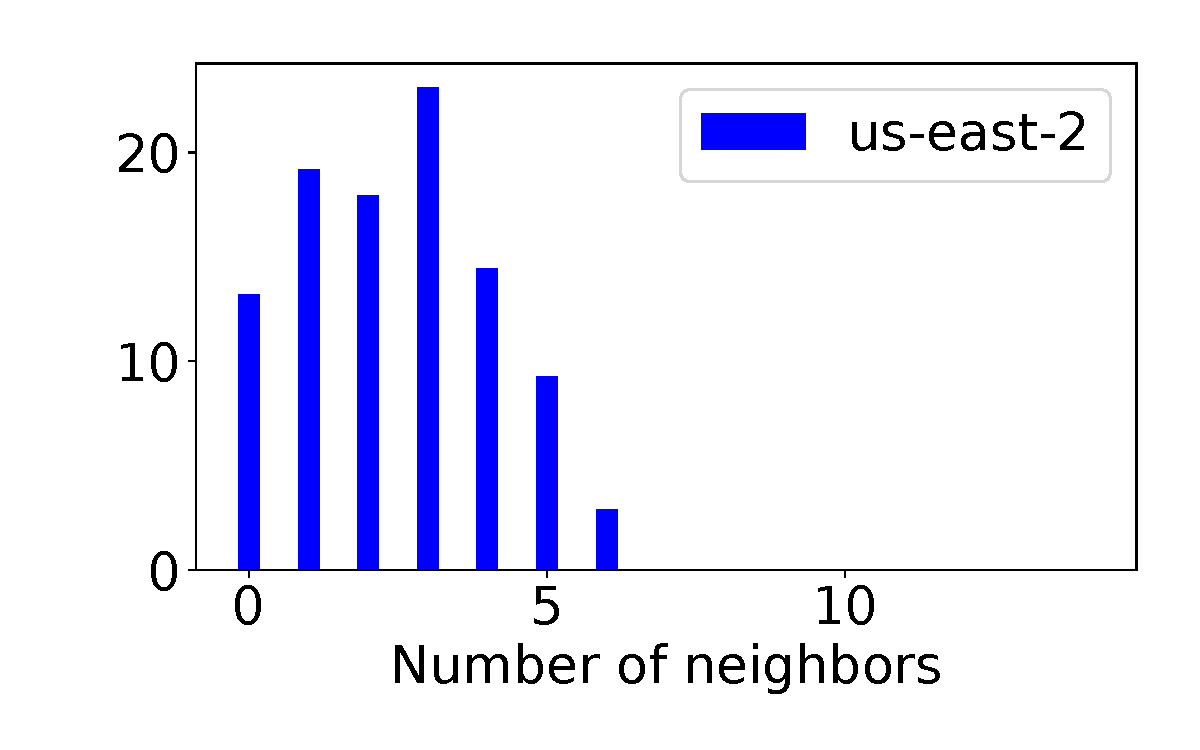
\includegraphics[width=.99\linewidth]{fig/colocation-us-east-2.pdf}
%   \caption{1b}
%   \label{fig:sfig2}
\end{subfigure}
\begin{subfigure}{.33\textwidth}
  \centering
  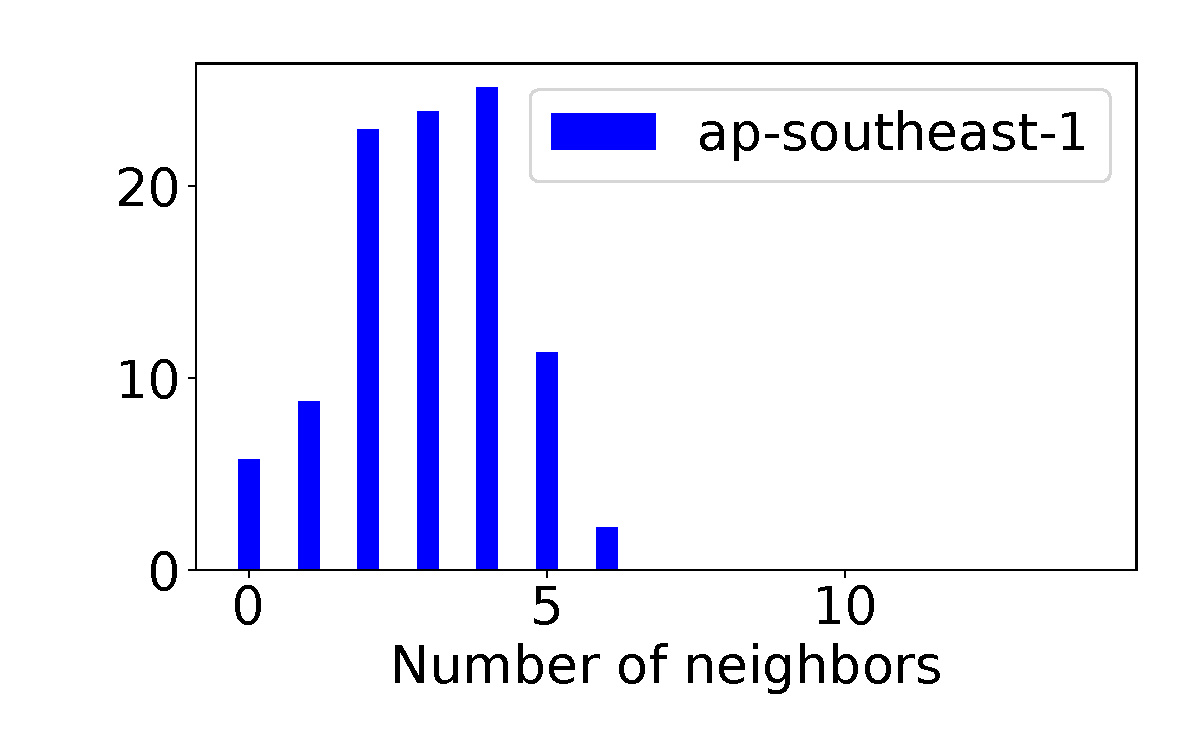
\includegraphics[width=.99\linewidth]{fig/colocation-ap-southeast-1.pdf}
%   \caption{1b}
%   \label{fig:sfig2}
\end{subfigure}

\begin{subfigure}{.33\textwidth}
  \centering
  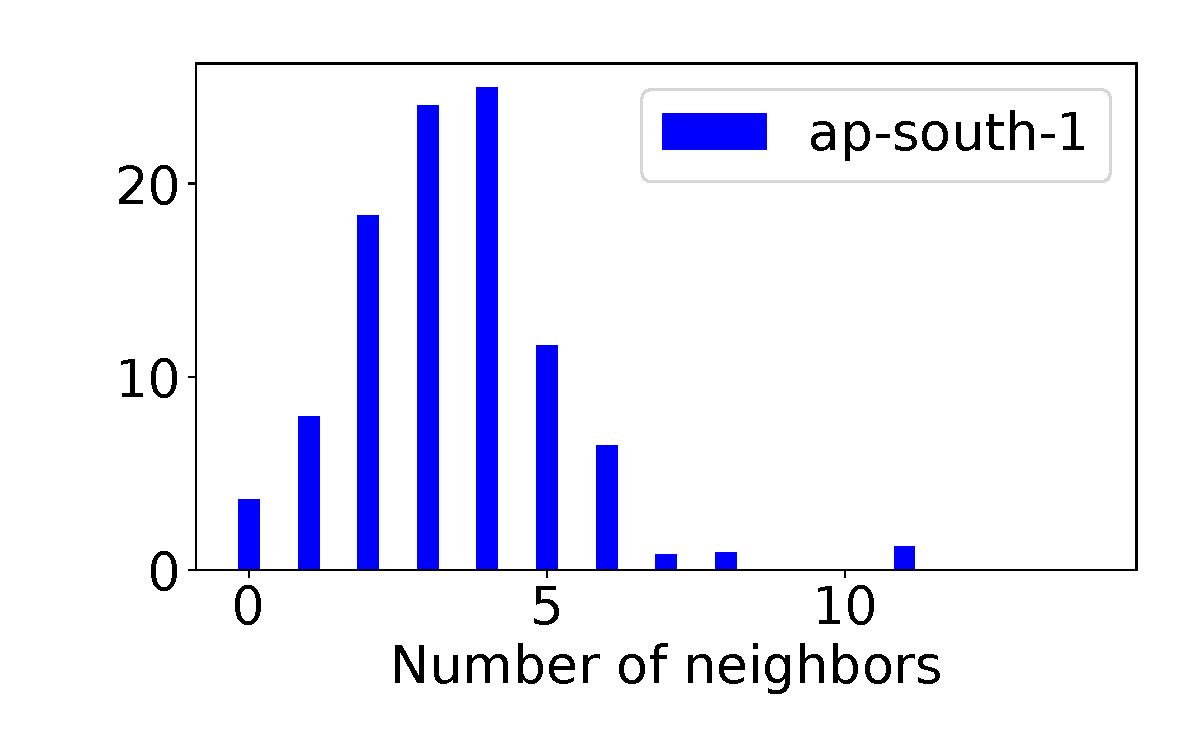
\includegraphics[width=.99\linewidth]{fig/colocation-ap-south-1.pdf}
%   \caption{1a}
%   \label{fig:sfig1}
\end{subfigure}%
\begin{subfigure}{.33\textwidth}
  \centering
  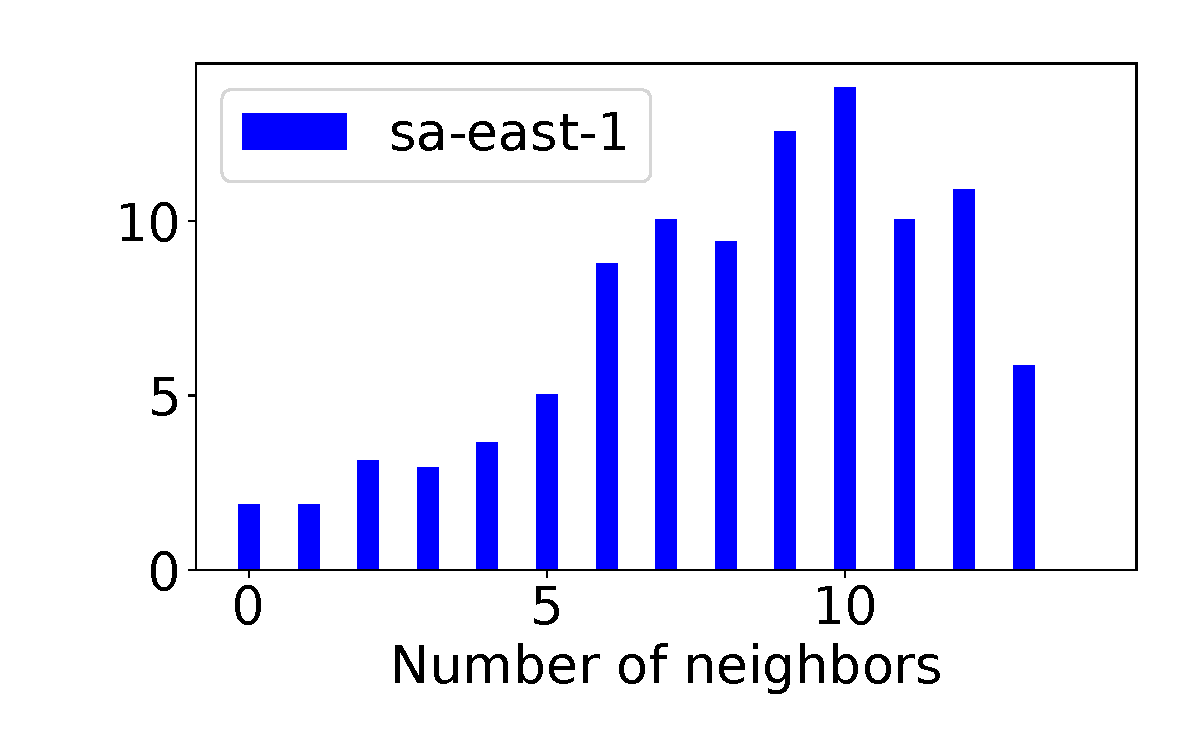
\includegraphics[width=.99\linewidth]{fig/colocation-sa-east-1.pdf}
%   \caption{1b}
%   \label{fig:sfig2}
\end{subfigure}
\begin{subfigure}{.33\textwidth}
  \centering
  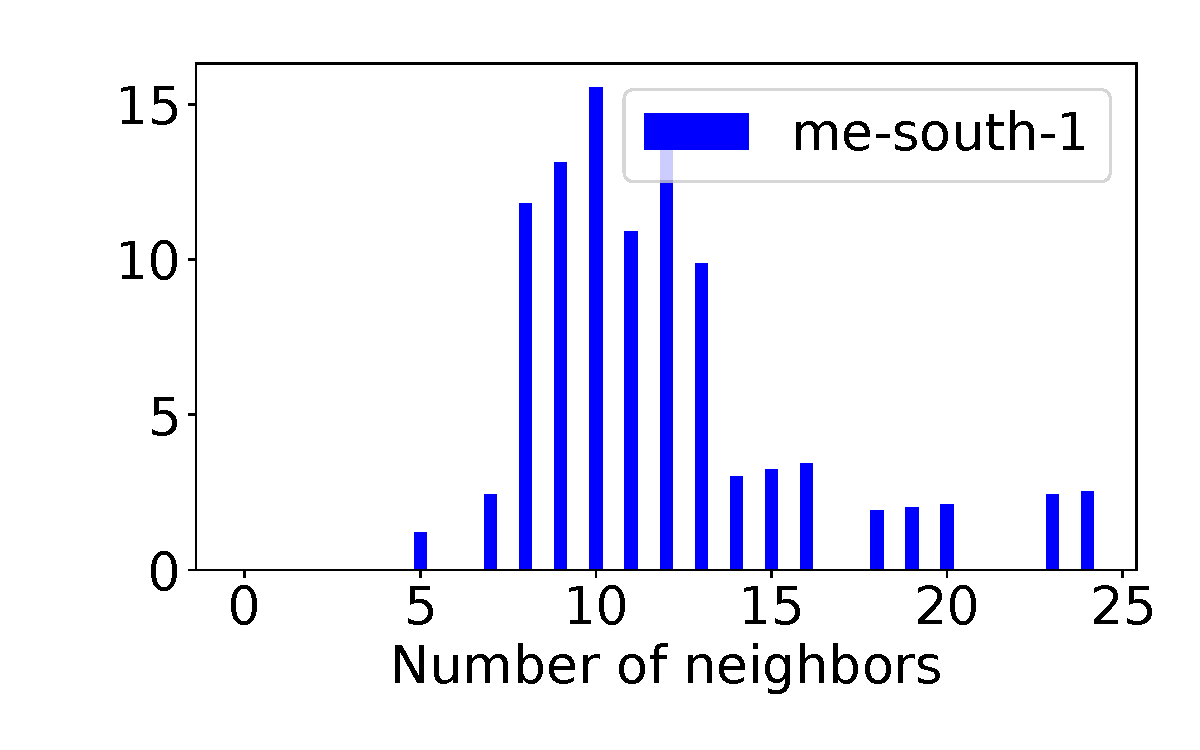
\includegraphics[width=.99\linewidth]{fig/colocation-me-south-1.pdf}
%   \caption{1b}
%   \label{fig:sfig2}
\end{subfigure}
\caption{Shows co-location results for a 1000-lambda run in different AWS regions. Each bar shows the fraction 
of those 1000 lambdas (in \%) that saw a certain number of neighbors. The total amount and density of co-location 
vary widely across regions, perhaps based on the size and lambda activity within those regions. }
\label{fig:awsregions}
\end{figure*}


%\paragraph{Generality}
%\todo{We only implemented it on AWS. This requires us to implement it on 
%Azure and GCP, and report some results. \textbf{Needs considerable effort}}
